\section{Diskussion der Ergebnisse}

\subsection{Durchlassfilter}
Beim Aufzeichnen der Spannungskurven für verschiedene Ohmsche Wiederstände fiel auf, dass die Maxima im Vergleich zu denen der Theoriekurven deutlich zu klein waren. Dabei wurde auch der an weiteren Bauteilen, hierbei vorallem die Spule, abfallende Widerstand berücksichtigt. Dieser wurde zuvor zu $ 3,0 \Omega $ ausgemessen (siehe Abb. \ref{plot:durchlass+R_ges}).\\
Abbildung \ref{plot:durchlass+R_ges-fit} zeigt die gleiche Messreihe, wobei hier über dem Gesamtwiderstand des Kreises als Variable gefittet wurde. Ergebnis war, dass dieser nochmals um etwa $ 4 \Omega $ größer ist, als zuvor im "Ruhezustand" gemessen. Grund hierfür ist wohl schlichtweg zusätzlicher Widerstand, der sich als Übergangswiderstand bei den Steckverbindungen ausbildet oder ein thermischer Widerstand in der Widerstandsbox.\\
Die geringen Abweichungen der Resonanzfrequenz, die überdies hinaus zu sehen sind, könnten unter anderem auf ungenaue Kapazitäts- und Induktivitätsangaben zurückgeführt werden, fallen allerdings kaum ins Gewicht.
\begin{figure}
        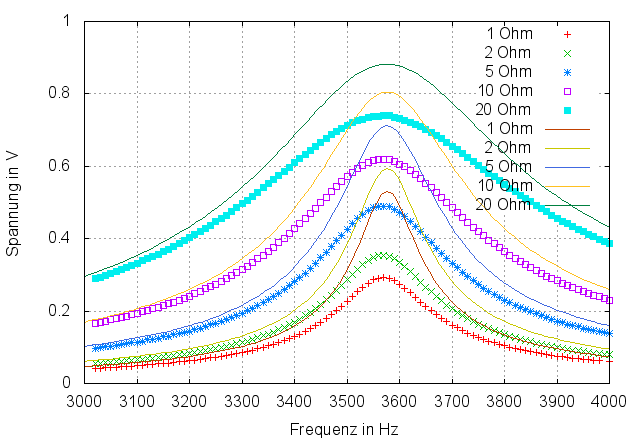
\includegraphics[width=.9\textwidth]{images/plot/durchlassfilter+theorie+R_ges.png}
\caption{Plot der Messdaten des Durchlassfilters (unter Vernachlässigung des Restlichen Wiederstandes)}
\label{plot:durchlass+R_ges}

	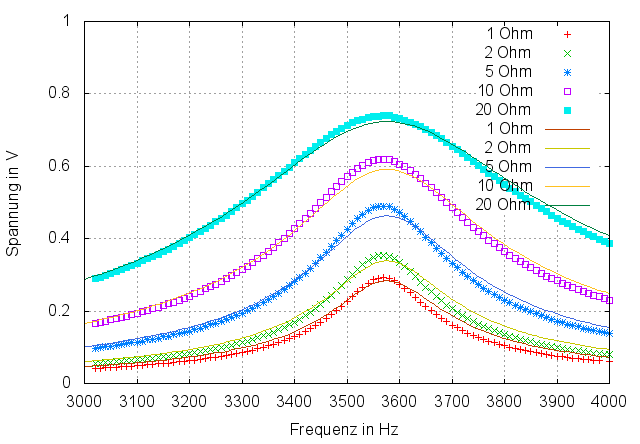
\includegraphics[width=.9\textwidth]{images/plot/durchlassfilter+theorie+R_ges-fit.png}
\caption{Plot der Messdaten des Durchlassfilters unter Berücksichtigung des gefitteten Gesamtwiederstandes}
\label{plot:durchlass+R_ges-fit}
\end{figure}
\subsection{Sperrfilter}
Ähnlich verhält es sich mit den aus dem Betrieb der zweiten Schaltung als Sperrfilter entstandenen Kurven (Abb. \ref{plot:sperr}). Nach Berücksichtigung des ohmschen Widerstandes der Spule ergeben sich nur noch minimale Abweichungen zwischen Theorie und den Messwerten, einzig die Resonanzfrequenz konnte nicht getroffen werden. Hier scheint es ebenfalls am warscheinlichsten, dass die Induktivität der zweiten Spule mit 36 mH nicht korrekt ist oder dass in anderen Bauteilen ungewollte Induktivitäten oder Kapazitäten auftreten.
\\
\begin{figure}[h]
        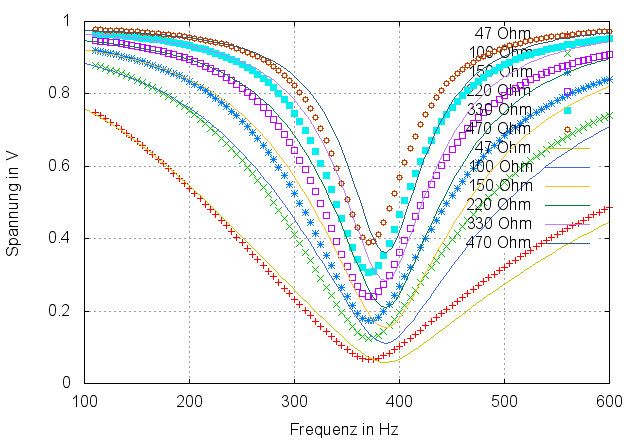
\includegraphics[width=.9\textwidth]{images/plot/sperrfilter+theorie+R_L.png}
\caption{Plot der Messdaten des Sperrfilters mit Theoriekurven}
\label{plot:sperr}
\end{figure}

\paragraph{}Vergleicht man also die Theorie der behandelten Frequenzfilter mit den tatsächlich gemessenen Ergebnissen, so stimmen beide vor allem in qualitativer Hinsicht gut überein. Durch Ersetzen von etwa der Widerstandsbox durch einen Schichtwiderstand, eine Reduktion des Widerstands der Spule sowie durch Löten der Kontake an Stelle von gewöhnlichen Steckverbindungen müssten darüberhinaus deutliche Verbesserungen möglich sein, was die Höhe des Spannungsverlaufs und dessen Abweichung von der Theorie betrifft. 
Darüber hinaus müsste es durch die Verwendung genauer ausgemessener Induktivitäten und Kapazitäten auch möglich sein, die Resonanzfrequenz besser zu treffen. 